\begin{frame}{Total Final World Energy Consumption}
	\begin{table}
		\centering
		\caption{Sector Percentage Shares of Balance Factors by Forman et al. \cite{forman2016estimating}}
		\begin{tabular}{cccc}
			\hline
			Sectors & Energy Service & Exhausts/Effluents & Other Losses\\
			\hline
			World & 28 & 52 & 20\\
			Electricity & 39 & 49 & 12\\
			Industrial & 49 & 30 & 21\\
			Commercial & 40 & 33 & 27\\
			Residential & 51 & 35 & 14\\
			Transportation & 19 & 59 & 22\\
			\hline
		\end{tabular}
	\end{table}
\end{frame}

\begin{frame}{IEA 2018 World Energy Balance}\label{worldenergybal}
	\begin{table}
		\centering
		\caption{2018 IEA World Energy Balance\cite{iea2018world}}
		 \begin{tabular}{ccc}
		 \hline
		 Sectors & Sector Percentage Share & Percent Losses\\
		\hline
		Electricity & 48.19 & 51.81 \\
		Industrial & 28.56 & --- \\
		Transportation & 29.09 & ---\\
		Non-energy & 9.24 & ---\\
		Other & 33.11 & --- \\
		\hline
		\end{tabular}
	\end{table}
\end{frame}

\begin{frame}{IEA 2018 Philippine Energy Balance}
	\begin{table}
		\centering
		\caption{2018 IEA Philippine Energy Balance\cite{IEA2018PhilippineEnergyBalance}}
		 \begin{tabular}{ccc}
		 \hline
		 Sectors & Sector Percentage Share & Percent Losses\\
		\hline
		Electricity & 29.24 & 70.76 \\
		Industrial & 22.55 & --- \\
		Transportation & 36.33 & ---\\
		Non-energy & 3.72 & ---\\
		Other & 37.39 & --- \\
		\hline
		\end{tabular}
	\end{table}
\end{frame}

\begin{frame}{DOE 2017 Philippines Energy Balance}
   \begin{table}
		\centering
		\caption{\centering 2017 Department of Energy (DOE) Total Final Energy Consumption by Sector Percentage Shares\cite{doe2017energysituationer}}
		 \begin{tabular}{cc}
			 \hline
			 Sectors & Percentage Shares \\
			 \hline
			 Transportation & 34.9 \\
			 Residential & 27.1 \\
			 Industrial & 23.5 \\
		     Commercial & 13.0 \\
			 Agriculture, Fishery and Forestry & 1.5 \\
			\hline
		  \end{tabular}
	\end{table}
\end{frame}

\begin{frame}{Sectoral Shares of Waste Heat Distribution}
	\begin{table}
		\centering
		\caption{\centering Percent Sectoral Shares of Waste Heat Distribution through Waste Heat Temperatures of $<100^{\circ}C$, $100-299^{\circ}C$ and $\geq300^{\circ}C$ by Forman et al. \cite{forman2016estimating}}
		\begin{tabular}{cccc}
			\hline
			Sectors & $<100^{\circ}C$ & $100-299^{\circ}C$ & $\geq300^{\circ}C$\\
			\hline
			World & 63 & 16 & 21\\
			Electricity & 88 & 12 & 0\\
			Industrial & 42 & 20 & 38\\
			Commercial & 59 & 5 & 36\\
			Residential & 36 & 64 & 0\\
			Transportation & 46 & 54 & 0\\
			\hline
		\end{tabular}
	\end{table}
\end{frame}

\begin{frame}{Sectoral Shares of Exergy Distribution}
	\begin{table}
		\centering
		\caption{\centering Percent Sectoral Shares of Exergy Distribution through Waste Heat Temperatures of $<100^{\circ}C$, $100-299^{\circ}C$ and $\geq300^{\circ}C$  by Forman et al. \cite{forman2016estimating}}
		\begin{tabular}{cccc}
			\hline
			Sectors & $<100^{\circ}C$ & $100-299^{\circ}C$ & $\geq300^{\circ}C$\\
			\hline
			World & 21 & 24 & 55\\
			Electricity & 35 & 65 & 0\\
			Industrial & 17 & 20 & 63\\
			Commercial & 22 & 8 & 70\\
			Residential & 16 & 84 & 0\\
			Transportation & 22 & 78 & 0\\
			\hline
		\end{tabular}
	\end{table}
\end{frame}

\begin{frame}{Heat Sources: 3 Thermal Stratification\cite{jouhara2018waste}}
		\begin{alertblock}{Low-Thermal Grade (Low-Enthalpy Grade)}
			Heat sources below $200^{\circ}Celsius$
		\end{alertblock}
	
		\begin{block}{Medium-Thermal Grade}
			Heat sources ranging from $200-400^{\circ}Celsius$
		\end{block}
		
		\begin{block}{High-Thermal Grade}
			Heat sources above $400^{\circ}Celsius$
		\end{block}	
\end{frame}

\begin{frame}{Low-Grade Thermal Sources: Exhaust Gas Temperature Range in Different  Thermal Processes by Bruckner et al\cite{bruckner2015industrial}}
    \begin{table}[]
        \centering
        \begin{tabular}{p{7.5cm}p{2.5cm}}
        \hline
        \textbf{Thermal Processes} &
        \textbf{Temp. Range ($^{\circ}C$)} \\
        \hline
     Exhaust gases exiting recovery devices in gas-fired boilers, ethylene furnaces, etc. &  70 - 230 \\
     Process steam condensate & 50 - 90 \\
     Cooling water from furnace doors & 30 - 50 \\
     Cooling water from annealing furnaces & 70 - 230 \\
     Cooling water from air compressors & 30 - 50 \\
     Cooling water from internal combustion engines & 70 - 120 \\
     Cooling water from air conditioning and refrigeration condensers & 30-40 \\
     Drying, baking, and curing ovens & 90 - 230 \\
     Hot processed liquids & 30 - 230 \\
     \hline
    \end{tabular}
    \end{table}
\end{frame}

\begin{frame}{Process Industries that have Low-Grade Thermal Sources by Bruckner et. al\cite{bruckner2015industrial}}
    \begin{columns}
        \column{0.45\textwidth}
		\begin{block}{Food and Beverage}
			Cleaning, Cooking, Pasteurizing, Whitening, Drying, Washing, Sterilizing, Boiling, Heat Treatment and Drainage
		\end{block}
		
		\begin{block}{Textile}
			Dry Heating, Ironing, Washing, Bleaching, Dyeing, Drying and Steaming
		\end{block}
		
		\begin{block}{Paper}
			Pulp and Paper Drying
		\end{block}
		
		\column{0.45\textwidth}
		\begin{block}{Chemical Process}
			Boiling, Distilling, and Various Chemical Processes
		\end{block}
		
		\begin{block}{Other Process Industries}
			Non-metallic mineral processes, Wood drying, Metal Cleaning and Paint Drying
		\end{block}
	\end{columns}
\end{frame}

\begin{frame}{Waste Recovery Technologies that uses Low Grade Thermal Sources\cite{jouhara2018waste}}
    \begin{enumerate}
        \item Economizer
        \item Rotary Regenerator
        \item Heat Pumps
        \item Recuperators
        \item Thermo Photovoltaic Generators
        \item Piezoelectric Power Generation
    \end{enumerate}
\end{frame}

\begin{frame}{2017 World Energy Council (WEC): World Energy Resources: Geothermal\cite{council2017world,WorldEnergyCouncil2013}}
\begin{itemize}
    \item Low-temperature geothermal resources in the world is about 140 EJ/yr of heat.
    \item World energy consumption is now about 420 EJ/yr.
\end{itemize}
$ 1 Exajoule (EJ) = 1 x 10^{8} Joules (J) = 2.778 x 10^{11} kW-hr$
\end{frame}

\begin{frame}{Geothermal Resource Type (GRT)\cite{white1975assessment}}
\begin{columns}
    \column{0.6\textwidth}
    \begin{enumerate}
        \item Convective Hydrothermal Resources 
            \begin{itemize}
                \item Vapor Dominated (VD)
                \item Liquid Dominated (LD)
            \end{itemize}
        \item Other Hydrothermal Resources 
            \begin{itemize}
                \item Sedimentary basin (SB)
                \item Geopressured (GP)
                \item Radiogenic (R)
            \end{itemize}
        \item Hot Rock Resources 
            \begin{itemize}
                \item Solidified or Hot-Dry Rock (HDR)
                \item Part Still Molten or Magma
            \end{itemize}
    \end{enumerate}
    \column{0.5\textwidth}
       \begin{table}
		\centering
		 \begin{tabular}{p{1cm}p{1.5cm}}
			 \hline
			 GRT & Temperature Range $^{\circ}C$ \\
			 \hline
			 VD & $\approx240$ \\
			 LD & 20-350 \\
			 SB & 20-150 \\
		     GP & 90-200 \\
			 R & 30-150 \\
			 HDR & 90-650 \\
			 Magma & $>600$\\
			\hline
		  \end{tabular}
	\end{table}
\end{columns}
\end{frame}

\begin{frame}{GRT: Convective Hydrothermal Resources:VD\cite{WorldEnergyCouncil2013}}
\begin{columns}
    \column{0.45\textwidth}
    \begin{figure}
        \centering
        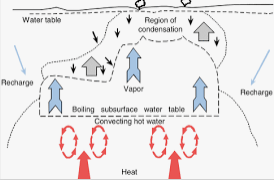
\includegraphics[height=4cm]{images/VDregion.png}
        \caption{\centering \scriptsize Vapor Dominated Resource\cite{lund2015worldwide}}
        \label{fig:vdr}
    \end{figure}
    \column{0.45\textwidth}
    \begin{figure}
        \centering
        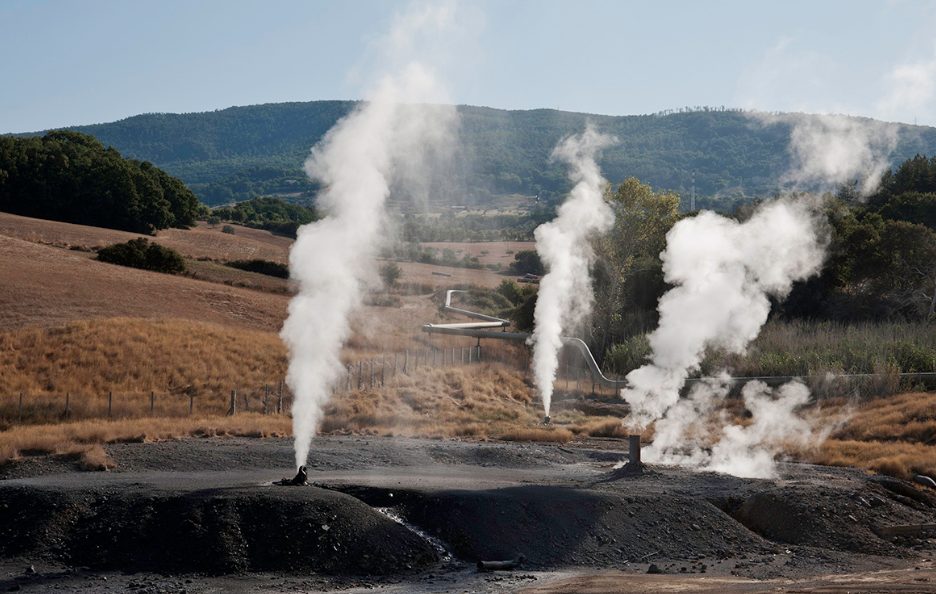
\includegraphics[height=2cm]{images/Lardello Italy.png}
        \caption{\centering \tiny Geysers at Larderello,Italy\cite{PaoloCagnacciPhotography}}
        \label{fig:larderello}
    \end{figure}
    \begin{figure}
        \centering
        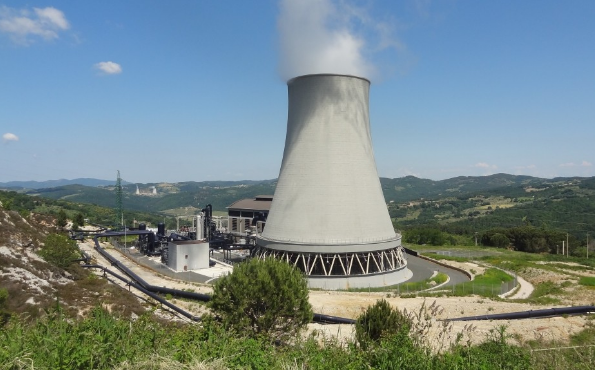
\includegraphics[height=2cm]{images/LarderelloGPP.png}
        \caption{\centering \tiny Sasso 2 geothermal plant by Enel Green Power, Tuscany, Italy (source: Volcanex)\cite{LarderelloGPP}}
        \label{fig:larderellogpp}
    \end{figure}
\end{columns}
\end{frame}

\begin{frame}{Power Station Energy Shares: Philippines}
   \begin{table}[h]
		\centering
		\caption{\centering 2018 IEA Phlippine Energy Balance - Power station energy shares\cite{IEA2018PhilippineEnergyBalance}}
		\label{tab:phppowerstationenergyshares}
		 \begin{tabular}{ccc}
			 \hline
			 Source of Energy & Percent Shares to Power Station \\
			 \hline
			 Oil Products & 2.50 \\
			 Coal & 51.06 \\
			 Natural Gas & 11.48 \\
		     Biofuels and Waste & 0.72 \\
			 \textbf{Geothermal} & \textbf{30.74} \\
			 Solar/Wind/Tide & 0.72 \\
			 Hydro & 2.78\\
			\hline
			Total & 100\% \\
			\hline
		  \end{tabular}
    \end{table}
\end{frame}

\begin{frame}{Geothermal Projected Capacities: Top Five Geothermal Power Producing Countries \cite{irenageothermalpower2017}}
    \begin{table}[h]
		\centering
		\caption{\centering Projected Geothermal Capacity (MW) for the Year 2016, 2025, and $>$2025}
		\label{tab:projectedgeothermalpower}
		\begin{tabular}{cccc}
			\hline
			 & 2016 & 2025 & $>$2025**\\
			\hline
			USA & 3490.3 & 3874.3 & 5425.3\\
			Indonesia & 1468.9 & 3410.7 & 4270.2\\
			\textbf{Philippines} & \textbf{1943.4} & \textbf{2104.4} & \textbf{2834.4}\\
			New Zealand & 1058.8 & 1128.8 & 1483.8\\
			Iceland& 612.4 & 752.4 & 1322.4\\
			\hline
		\end{tabular}
		\caption{\centering** Capacity additions after 2025 correspond to planned and deferred projects without completion date}
	\end{table}
\end{frame}

\begin{frame}{DOE Project: Detailed Assessment of Selected Low Enthalpy Geothermal
Resources in the Philippines\cite{halcon2015detailed}}
    \begin{alertblock}{Primary Objective}
        Accelerate the development of  of Low to Medium
        Enthalpy Geothermal Resource Area, with a temperature ranging from 90$^{\circ}$C - 150$^{\circ}$C, mainly for power generation.
    \end{alertblock}
    \begin{block}{Secondary Objectives}
         Assessment and realization of the economic feasibility of small scale geothermal power projects for local power needs.
    \end{block}
    \begin{block}{Secondary Objectives}
        Prepares of a comprehensive data package that will showcase this type of geothermal resource for future private investors.
    \end{block}
\end{frame}

\begin{frame}{DOE Project: Detailed Assessment of Selected Low Enthalpy Geothermal
Resources in the Philippines\cite{halcon2015detailed}}
    \begin{block}{Identified Low Enthalpy Gesource Resource Areas}
        Banton Island, Romblon
    \end{block}
    \begin{figure}
        \centering
        
\includegraphics[height=2.5cm]{images/DOEbontonisland.PNG}
        \caption{\centering Conducting Geological, Geochemical and Controlled Surface Magneto Telluric (CSMT) Survey at Banton Island, Romblon}
    \end{figure}
\end{frame}

\begin{frame}{DOE Project: Detailed Assessment of Selected Low Enthalpy Geothermal
Resources in the Philippines\cite{halcon2015detailed}}
    \begin{block}{Identified Low Enthalpy Gesource Resource Areas}
        Maricaban (Tingloy) Island, Batangas (left figure) \\
        Balut Island, Davao del Sur (right figure)
    \end{block}
    \begin{figure}
        \centering
        
\includegraphics[height=2.5cm]{images/DOEmaricaban.PNG}
        \caption{\centering \small Conducting Geological, Geochemical and CSMT Survey at Maricaban (Tingloy Island), Batangas and Balut Island, Davao Oriental}
    \end{figure}
\end{frame}

\begin{frame}{Tingloy Island Geothermal Wells}
    \begin{columns}
    \column{0.45\textwidth}
    \begin{table}[h]
        \centering
        \caption{Tingloy Geothermal Well Data}
        \begin{tabular}{ccc}
        \hline
            Slim Well &  Type of Well & Depth (m) \\
            \hline
             SH01 & Production & 490-500 \\
             SH02 & Reinjection & 1000-1015 \\
             \hline
        \end{tabular}
        \label{tingloywells}
    \end{table}
    \begin{table}[h]
        \centering
        \begin{tabular}{cp{2cm}p{1.75cm}}
        \hline
            Slim Well & Wellhead Pressure (kPa) & Wellhead Temperature ($^\circ$C)\\
            \hline
             SH01 & 4,820-4,860 & 120-130 \\
             SH02 & 9,600-9,610 & 130-140 \\
             \hline
        \end{tabular}
    \end{table}
    \column{0.45\textwidth}
    \begin{figure}
        \centering
        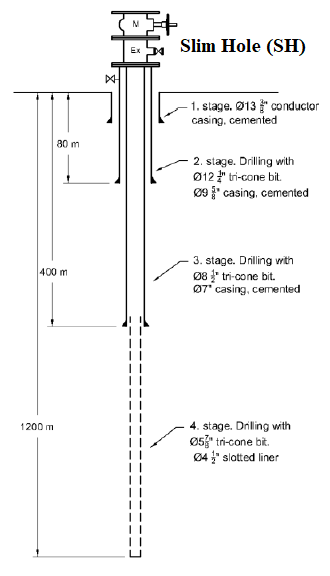
\includegraphics[height=4cm]{images/slimhole1.png}
        \caption{\centering Slim Wells used for Production and Reinjection Wells \cite{thorhallsson2012slim}}
        \label{fig:slimwells}
    \end{figure}
    \end{columns}
\end{frame}

\begin{frame}{NOHTFPECGPPIE Geothermal Wells using Tingloy Data from DOE\cite{halcon2015detailed}}
    \begin{figure}
        \centering
        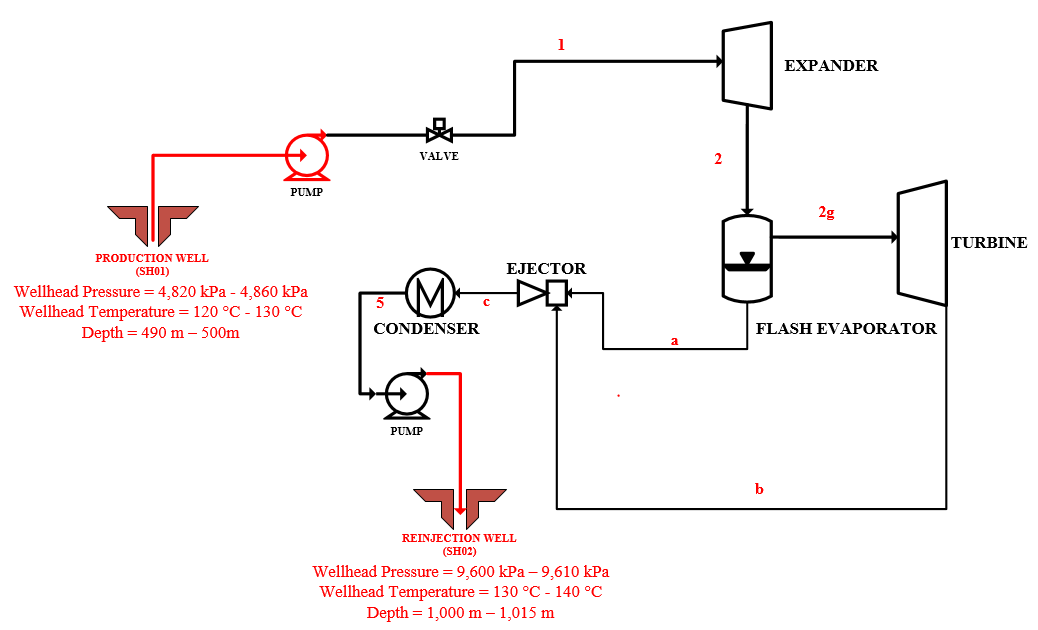
\includegraphics[height=0.4\textwidth]{images/nohtfpecgppiewells.png}
    \end{figure}
\end{frame}

\begin{frame}{Tingloy Geothermal Well Brine Density Readings for SH01 - First Test\cite{halcon2015detailed}}
    \begin{columns}
    \column{0.45\textwidth}
    \begin{figure}
        \centering
        \caption{\centering First Run Down Test}
        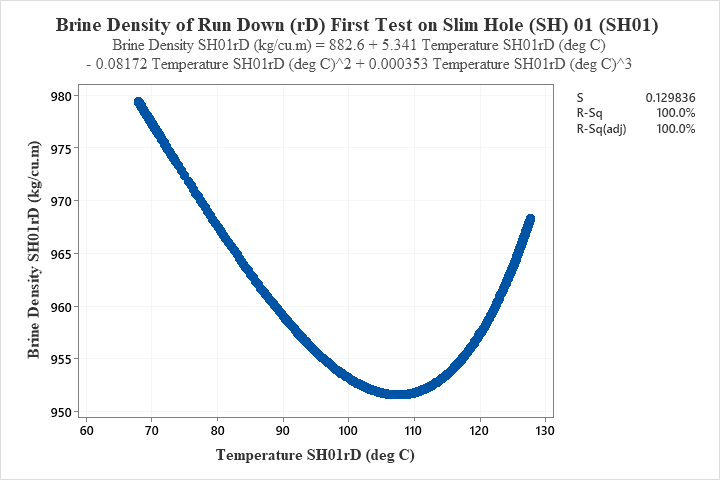
\includegraphics[height=4cm]{images/sh01r1d.png}
    \end{figure}
    \column{0.45\textwidth}
    \begin{figure}
        \centering
        \caption{\centering First Run Up Test}
        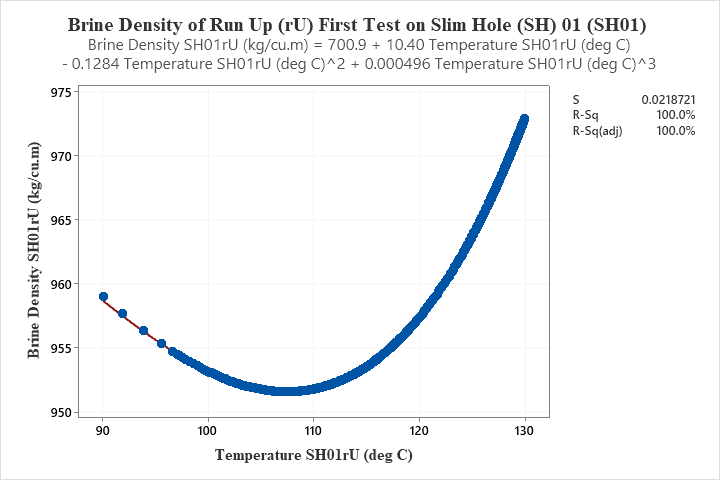
\includegraphics[height=4cm]{images/sh01r1u.png}
    \end{figure}
    \end{columns}
\end{frame}

\begin{frame}{Tingloy Geothermal Well Brine Density Readings for SH01 - 2nd Test\cite{halcon2015detailed}}
    \begin{columns}
    \column{0.45\textwidth}
    \begin{figure}
        \centering
        \caption{\centering Second Run Down Test}
        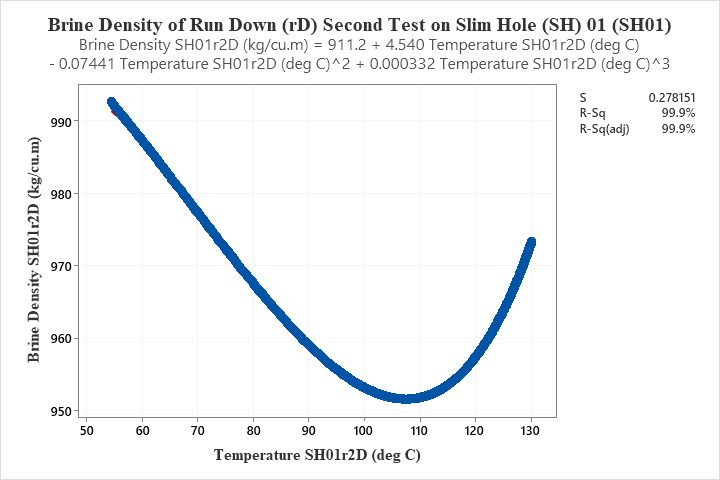
\includegraphics[height=4cm]{images/sh01r2d.png}
    \end{figure}
    \column{0.45\textwidth}
    \begin{figure}
        \centering
        \caption{\centering Second Run Up Test}
        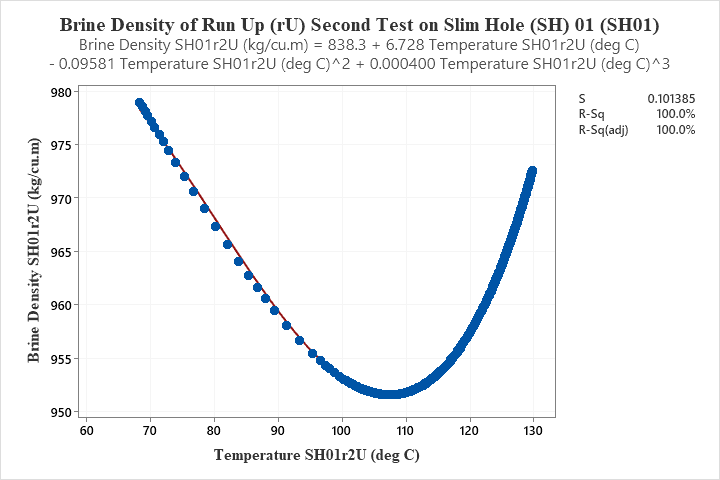
\includegraphics[height=4cm]{images/sh01r2u.png}
    \end{figure}
    \end{columns}
\end{frame}

\begin{frame}{Tingloy Geothermal Well Brine Density Readings for SH01 - 3rd Test\cite{halcon2015detailed}}
    \begin{columns}
    \column{0.45\textwidth}
    \begin{figure}
        \centering
        \caption{\centering Third Run Down Test}
        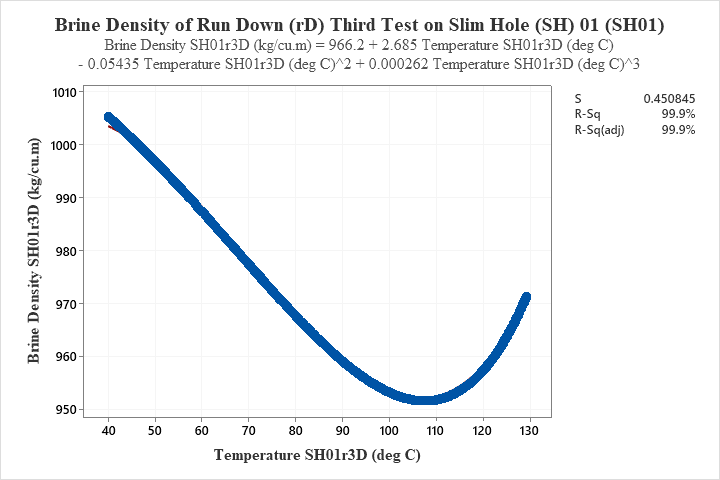
\includegraphics[height=4cm]{images/sh01r3d.png}
    \end{figure}
    \column{0.45\textwidth}
    \begin{figure}
        \centering
        \caption{\centering Third Run Up Test}
        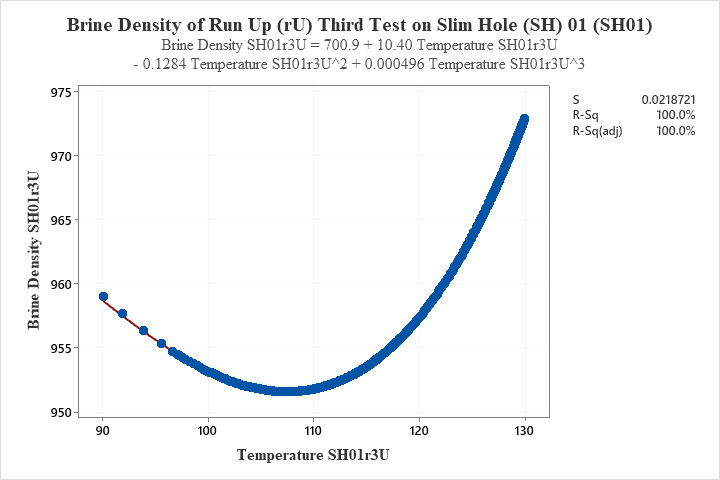
\includegraphics[height=4cm]{images/sh01r3u.png}
    \end{figure}
    \end{columns}
\end{frame}

\begin{frame}{Types of Expansion Devices Based on Working Principles\cite{smith2014power}}
   \begin{columns}
   \column{0.45\textwidth}
   \begin{enumerate}
        \item Turbine or Turbo Expanders
            \begin{itemize}
                \item Radial Inflow
                \item Radial Outflow
                \item Axial
            \end{itemize}
        \item Positive Displacement
            \begin{itemize}
                \item Scroll
                \item Screw
                \item Rotary Vane
                  \begin{itemize}
                    \item Wankel
                  \end{itemize}
                \item Piston
                \item Roots
            \end{itemize}
        \item Ejector
    \end{enumerate}
    \column{0.45\textwidth}
    \begin{figure}
        \centering
        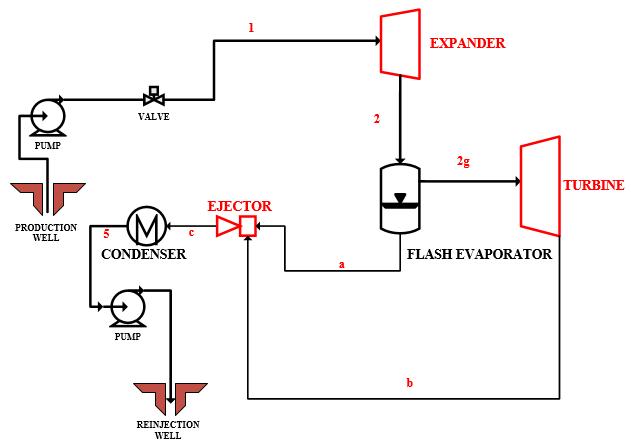
\includegraphics[height=4.5cm]{images/nohtfpecgppiexd.png}
        \caption{\centering \scriptsize NOHTFPECGPPIE emphasizing expansion devices}
    \end{figure}
   \end{columns}
\end{frame}

\begin{frame}{Expander}
	\begin{table}[h]
		\centering
		\caption{\centering Capacity Ranges, Rotative Speeds and Costs of the Different Types of Expander Installed in an Organic Rankine Cycle\cite{pethurajan2018issues}}
		\label{tab:expandercapacityinORC}
		\begin{tabular}{|p{3.75cm}|p{2cm}|p{2.5cm}|p{1.5cm}|}
			\hline
			Type & Capacity Range (kW) & Rotative Speed (rpm) & Cost\\
			\hline
			Radial-Inflow Turbine & 50-500 & 8,000-80,0000 & High\\
			Scroll Expander & 1-10 & $<6,000$ & Low\\
			Screw Expander & 15-200 & $<6,000$ & Medium\\
			Rotary Vane Expander & 1-10 & $<6,000$ & Low\\
			\hline
		\end{tabular}
	\end{table}
\end{frame}

\begin{frame}{Expander}
    \begin{table}[h]
		\centering
		\caption{\centering Advantages and Disadvantages of the Different Types of Expander Installed in an Organic Rankine Cycle\cite{pethurajan2018issues}}
		\label{tab:expanderadvanddisadvinorc}
		\begin{tabular}{p{3cm}p{3.5cm}p{3.5cm}}
			\hline
			Type & Advantages & Disadvantages\\
			\hline
			Radial-Inflow Turbine & Lightweight with High efficiency & Cannot bear two-phase flow \\
			Scroll Expander & High efficiency, lightweight, low rotating speed and Tolerable two-phase flow & Requires lubrication and modification \\
			\hline
		\end{tabular}
	\end{table}
\end{frame}

\begin{frame}{Expander}
    \begin{table}[h]
		\centering
		\caption{\centering Advantages and Disadvantages of the Different Types of Expander Installed in an Organic Rankine Cycle\cite{pethurajan2018issues}}
		\label{tab:expanderadvanddisadvinorc}
		\begin{tabular}{p{3cm}p{3.5cm}p{3.5cm}}
			\hline
			Type & Advantages & Disadvantages\\
			\hline
			Screw Expander & Tolerable two-phase flow, low rotating speed and high efficiency & Requires lubrication \\
			Rotary Vane Expander & Tolerable two-phase flow, stable torque, simple structure, low cost and noise & Requires lubrication and low capacity \\
			\hline
		\end{tabular}
	\end{table}
\end{frame}

\begin{frame}{Scroll Expander: Operating Conditions}
    \begin{table}[h]
    \centering
    \caption{Operating Conditions of a Scroll Steam Expander\cite{kim2007scroll}}
    \label{tab:scrollexpanderopcond}
    \begin{tabular}{p{2cm}p{2.5cm}p{2.5cm}p{2.5cm}}
    \hline
        Shaft speed (rpm) & Inlet Pressure (kPa) & Outlet Pressure (kPa) & Inlet Temperature ($^{\circ}$C) \\
    \hline
         1,384 & 1,201.6 & 114.0 & 139 \\
         1,205 & 1,199.7 & 112.8 & 143 \\
         1,130 & 1,236.0 & 113.6 & 144 \\
         1,011 & 1,301.7 & 113.7 & 145 \\
    \hline
    \end{tabular}
\end{table}
\end{frame}

\begin{frame}{Selections of Steam Expander based on criteria for Low-Power Rankine Cycle\cite{badr1991expansion}}
    \begin{table}[h]
    \centering
    \label{tab:steamexpanderselection}
    \begin{tabular}{p{3cm}p{1.25cm}p{1.25cm}p{1.25cm}p{1.225cm}p{1.5cm}}
    \hline
        Targets & Turbines & R.Piston & Helical-Screw & Rotary Vane & Wankel \\
    \hline
         5-20 kW\textsuperscript{1} & No & Yes & Yes & Yes & Yes \\
        3,000-5,000 rpm\textsuperscript{2} & No & Yes & Yes & Yes & Yes \\
        $65-75\%\textsuperscript{3}$ & No & No & Yes & Yes & Yes \\
        Two-phase flow\textsuperscript{4} & No & Low & Yes & Yes & Yes \\
        Lubrication\textsuperscript{5} & --- & --- & No & Yes & No \\
    \hline
    \end{tabular}
    \caption{\scriptsize 1 = Low power output in kiloWatts, 2 = Low rotational speed in revolutions per minute (rpm), 3 = Isentropic Expander Efficiency, 4 = Ability of the expander to allow wet expansion without adverse effect on the performance and life of the expander(i.e. can handle two-phase flow expansion), 5 = Lubrication Problems during operation.}
    \end{table}
\end{frame}

\begin{frame}{Performance Map for Different Types of Expander\cite{badr1991expansion}}
\begin{figure}
    \centering
    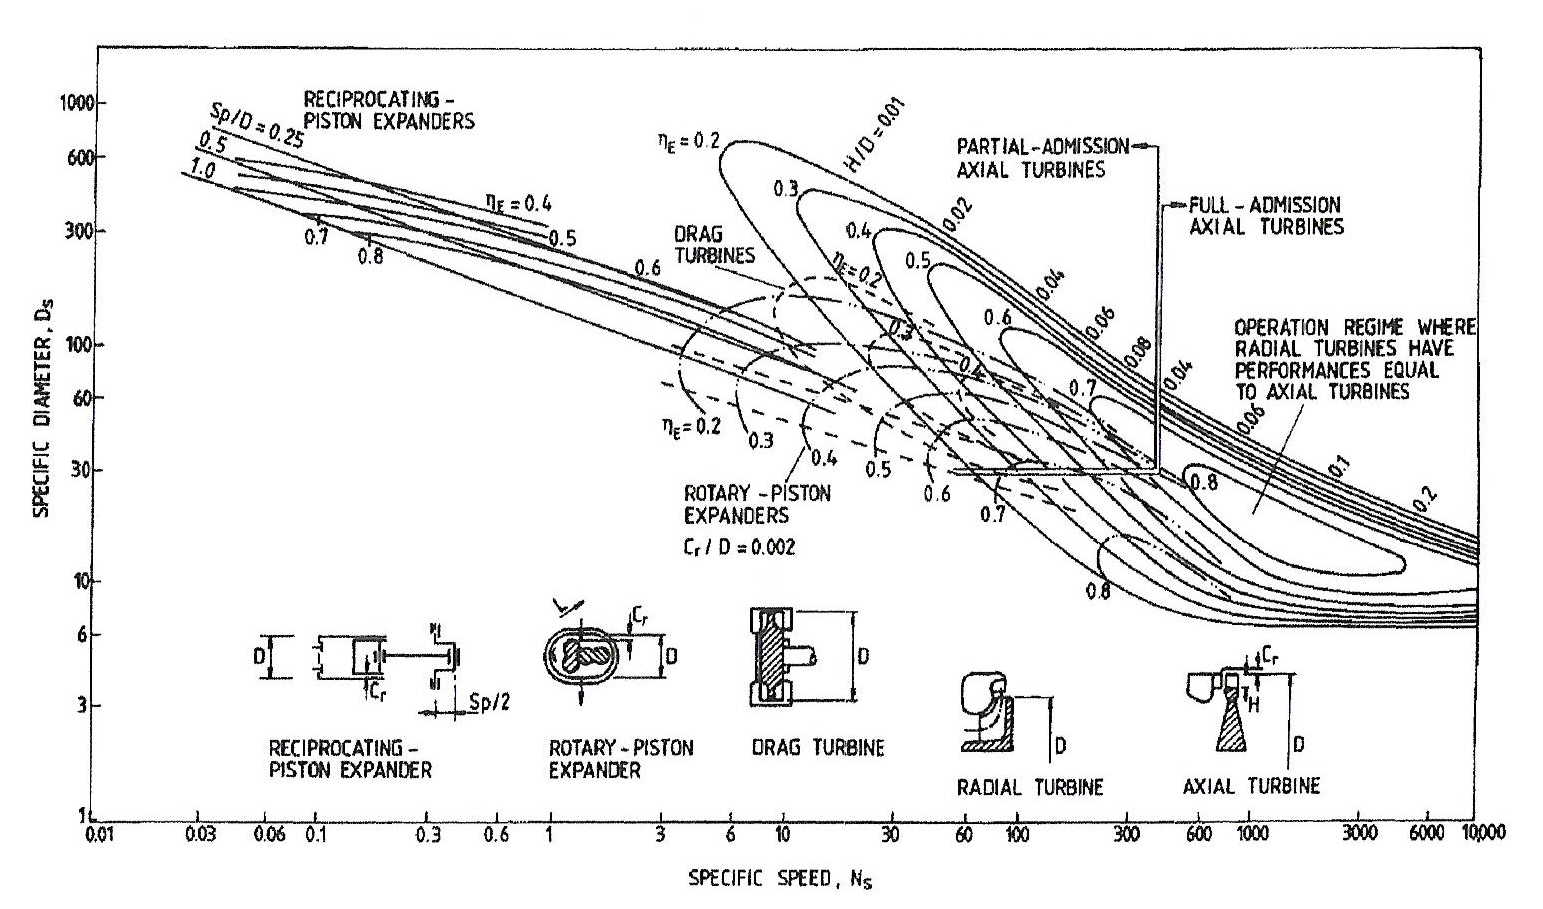
\includegraphics[height=6.25cm]{images/Expander1.png}
    \label{fig:expanderperformancetype}
\end{figure}
\end{frame}

\begin{frame}{Use of Expanders in Trilateral Flash Cycle (TFC)}
    \begin{block}{Cipollone et al. 2017 \cite{cipollone2017low}}
     \begin{itemize}
         \item Remarks: Novelty of the research is the use of \textbf{rotary positive displacement expander}
         \begin{itemize}
             \item Findings: R1234z(E) and propane provides a greater specific work, however, it would require built-in  \textbf{volume ratios of 8 and 14}, respectively, which is \textbf{beyond the capabilities of rotary positive displacement which is 5}.
         \end{itemize}
         \item Cycle: Trilateral Flash Cycle (TFC)
         \item Analysis: Thermodynamic Analysis
         \item Working Fluids: R1234yf, R1234z(E), R134a, Propane, Cyclopropane, R1234zE/CO2 (0.9/0.1), Propane/CO2 (0.9/0.1), Propane/CO2 (0.8/0.2), Propane/CO2 (0.7/0.3)
         \item Working Temperatures: Heat Source Temperature of 100$^{\circ}C$ and Heat Sink Temperature of 40$^{\circ}C$
     \end{itemize}
    \end{block}
\end{frame}

\begin{frame}{Converted Scroll Compressor into Expanders\cite{zhao2019expansion}}
    \begin{table}[h]
        \centering
        \begin{tabular}{cp{2.5cm}p{2.25cm}p{2.5cm}c}
        \hline
            Working Fluid & Output Power (kW) & Expansion Ratio & Rotational Speed (rpm) & Efficiency (\%) \\
            \hline
            R123 & 1.54 & 3.84 & 2,165 & 86 \\
            R123 & 0.75 & --- & 2,100 & 38 \\
            R245fa & 2.3 & 5.2 & 2,970 & 73 \\
            R245fa & 1.8 & 2-7 & 3,500 & 75.7 \\
            R123 & 2.78 & --- & --- & 85.17 \\
            R245fa & --- & 4.58 & 3,000 & 84.9 \\
            R245fa & 1.016 & 10.68 & 3,496 & 77.74 \\
            R123 & --- & --- & 3,000 & --- \\
            R134a & 0.557 & 3.6 & 3,450 & 78 \\
            R245fa & 3.75 & --- & 3,500 & 58 \\
            \hline
        \end{tabular}
    \end{table}
\end{frame}